\documentclass[12pt,a4paper]{article}

\usepackage[utf8]{inputenc}
\usepackage{lmodern}
\usepackage[T1]{fontenc}
% paysage
% \usepackage[landscape]{geometry}
\usepackage{lscape}
\usepackage{graphicx}
% \graphicspath{ {images/} }

% headers footers
\usepackage{fancyhdr}
\pagestyle{fancy}

% référencer la dernière page
\usepackage{lastpage}

% pdf
\usepackage{pdfpages}

% francais
\usepackage[frenchb]{babel}
% math
\usepackage{amssymb}

\usepackage{multicol}
\usepackage{url}

\usepackage{multido}
\usepackage[utf8]{inputenc}
% \usepackage{lmodern}
\usepackage[T1]{fontenc}

\usepackage[sfdefault]{AlegreyaSans} %% Option 'black' gives heavier bold face
%% The 'sfdefault' option to make the base font sans serif
% \renewcommand*\oldstylenums[1]{{\AlegreyaSansOsF #1}}

\usepackage{breqn}
\usepackage{multicol}
\usepackage[frenchb]{babel}
% \usepackage{pstricks,pst-plot,pst-node}
% \usepackage{pstricks-add}
\usepackage{pst-circ}
\usepackage{pst-magneticfield}
\usepackage{pst-electricfield}
\usepackage{graphicx}
\usepackage{amsmath,amsfonts,amssymb}
\usepackage{titlesec} 
\usepackage{float}
\usepackage{textcomp}
\usepackage{amssymb}
\usepackage[toc,page]{appendix}
\usepackage{listings} 

\lstset{language=Matlab}
\usepackage{lipsum}
\usepackage{enumerate}


%Numerotation par section des équations
\usepackage{amsmath}

\usepackage{tabularx}
\usepackage{longtable}

%------------------------------inclue les références
% \usepackage[nottoc, notlof, notlot]{tocbibind}
%\usepackage{biblatex}
% \usepackage{csquotes}

%\usepackage{etoolbox}
% \patchcmd{\chapter}{\thispagestyle{plain}}{\thispagestyle{fancy}}{}{}
\title{
	\Huge\textsc{Geographic coordinates}
}
\author{Mohamed Thebti} 

\begin{document}
% retrait de la première ligne d'un paragraphe
\setlength{\parindent}{0mm}

\fancyhead[R]{\slshape \leftmark}
\fancyhead[L]{\slshape Geographic coordinates}
%\fancyhead[LE,RO]{\slshape \rightmark}
% \fancyhead[LO,RE]{\slshape \leftmark}

% \fancyfoot[C]{Travail de Master}
\fancyfoot[L]{\slshape Mohamed Thebti}
\fancyfoot[C]{}
\fancyfoot[R]{\thepage}

\maketitle
\newpage

\tableofcontents

\newpage



\section{Introduction}

The objective of this report is to compute real distance between two points on the globe. This question is important because people are used to use map, which makes them forget the spherical shape of the planet.

The following picture\footnote{\url{https://justglobes.uk/oxford-desktop-globe.html}} is showing the view on the planet from space. \\

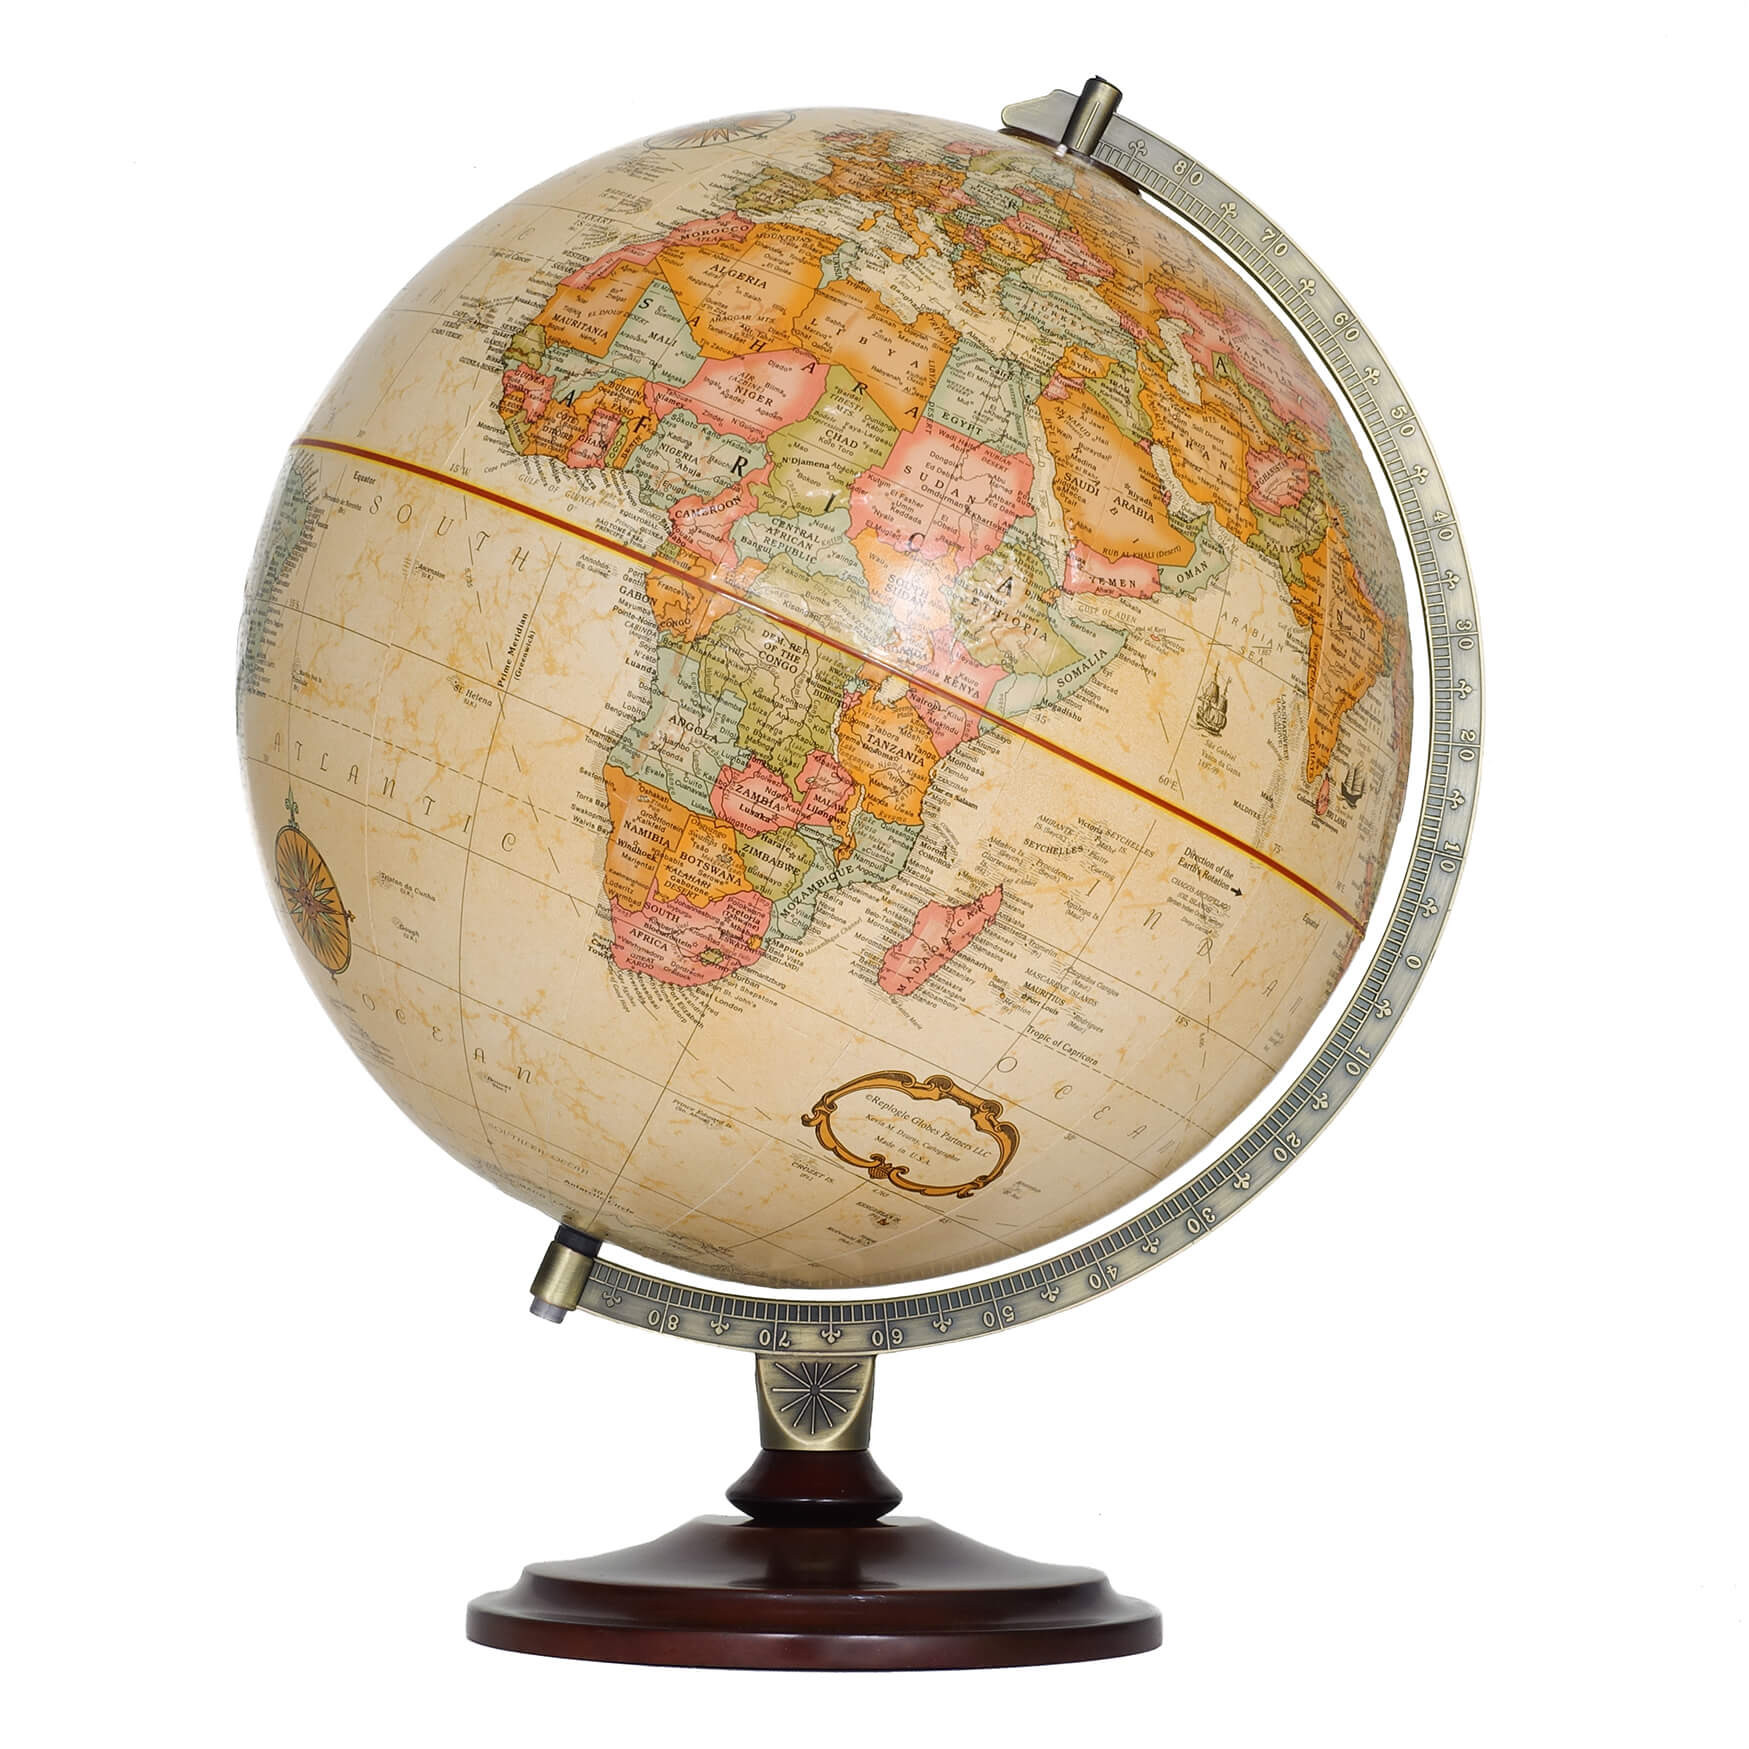
\includegraphics[scale=.2]{oxford-2021-01.jpg}

\newpage
\section{Conversion of degrees to distance}
Because of the spherical shape of the planet, the length of a degree is different, according to the position of the observer on the globe. This means that  
if a traveler wants to move between two points situated at a distance of 1 degree from each other, for example 36° and 37°, he will have to walk a different distance, if he is near the Equator or on the North/South Pole \footnote{\url{https://en.wikipedia.org/wiki/Geographic_coordinate_system}}.


At latitude between $\phi$ and $\phi+1$, 1 degree latitude is equal in meters to:
\begin{dmath}
	L_{latitude}(\phi) = 111'132.92-559.82 \cdot cos(2 \phi) + 1.175 \cdot cos(4\phi) \\ -0.0023 \cdot cos(6\phi)
\end{dmath}

At a specified latitude $\phi$, each longitude degree is equal to : 
\begin{dmath}
	L_{longitude}(\phi) =
111'412.84-93.5 \cdot cos(3\phi)+ 0.118 \cdot cos(5\phi)
\end{dmath}
\subsection{Example}

Let's consider the following location on Earth : $\phi = 35.3\degres$,  $\lambda = 42.8\degres$.
we want to compute the distance in meter that we must travel.
Starting from the intersection of the Equator and the Greenwitch longitude ($\phi = 0\degres$,  $\lambda = 0\degres$), we move north (latitude increasing)

From $\phi = 0\degres$ to $\phi = 35\degres$, we compute the length of each degree and we sum them together. For the last $0.3\degres$, compute the length at $\phi = 36\degres$ then we multiply it with the remaining decimal.
\begin{equation}
	L_{latitude}^{total} = \sum_{\phi=0}^{34}  L_{latitude}(\phi) + L_{latitude}(\phi=35.3)
\end{equation}

\begin{table}[ht]
	\caption{Latitude distance} % title of Table
	\centering % used for centering table
	\begin{tabular}{c c } % centered columns (4 columns)
		\hline\hline %inserts double horizontal lines
		Latitude [°] & Distance [m] \\ [0.5ex] % inserts table
		%heading
		\hline % inserts single horizontal line
		0 & 110'574.27 \\ % inserting body of the table
		1 & 110'574.61 \\
		... &  \\ 
		34 & .... \\
		35.3 & ... \\ 
		[1ex] % [1ex] adds vertical space
		\hline %inserts single line
	\end{tabular}\label{table:nonlin} % is used to refer this table in the text
\end{table}

At this latitude, we need to move East to reach our target location. 

We use the same method to compute the longitude distance at $\phi=35.3\degres$. 

\begin{dmath}
	L_{longitude}^{total} = 42.8 * L_{longitude}(35.3\degres) = 42.8 * 111'438.34  = 4'769'500.176 m = 4'769.5 km
\end{dmath}

\newpage


\end{document}